\chapter{Our Methodology and Approach}
\label{chap:methodology}

This chapter describes the methodology followed during the internship. The approach is organized around two generative pipelines: a baseline diffusion model in physical image space and a wavelet-based diffusion model using multi-resolution coefficients.

\section{DNS dataset and preprocessing}

The reference data used in this work are generated by Direct Numerical
Simulations of the Rayleigh--Taylor instability. This choice is motivated by
the need for high-fidelity fields: lower-fidelity turbulence models may be
useful in other contexts, but they introduce closure assumptions that are not
desirable here because the objective is precisely to learn the distribution of
physically resolved density fields.

The simulations are produced with a pseudo-spectral solver on two-dimensional
periodic domains initialized with perturbed density interfaces. Each stored
sample corresponds to a snapshot of the temporal evolution of the instability.
The resulting fields contain both large coherent structures and fine
interfacial fluctuations, which makes them relevant for both direct and
multi-resolution generative modeling.

Although DNS provide high-fidelity information, their computational cost
remains substantial because all dynamically relevant scales must be resolved.
As a consequence, the available dataset is relatively small: it is built from
roughly 60 independent simulations and, after preprocessing and filtering,
contains fewer than 7000 images split into training, validation, and test
subsets. This limited size is an important methodological constraint because it
increases the risk of overfitting and reduces the diversity available to the
generative models.

\subsection{Geometric constraints and cropping}

Unlike generic computer vision datasets, the geometry of the raw RTI fields is
not arbitrary. The horizontal direction is periodic, so the domain width must
remain large enough to prevent the largest coherent structures from interacting
too strongly with their periodic images. If $L_x$ denotes the horizontal
domain size and $L_b$ the diameter of the largest bubbles, one seeks to remain
in a regime such that

\begin{equation}
    L_b \ll L_x,
\end{equation}

or more conservatively

\begin{equation}
    L_b \lesssim \frac{L_x}{4}.
\end{equation}

The vertical direction follows a different constraint because the mixing layer
grows under gravity and therefore requires a longer observation window. The raw
simulations are consequently produced on domains of size $128\times512$.

Since the baseline model is trained on square inputs, the original fields are
cropped to a square field of view. This cropping is retained only when the full
mixing zone remains inside the selected window. Let $y_b(t)$ and $y_s(t)$
denote the lowest bubble tip and the highest spike tip. The retained crop must
satisfy

\[
y_{\min}^{\mathrm{crop}} < y_b(t)
\quad\text{and}\quad
y_s(t) < y_{\max}^{\mathrm{crop}},
\]

so that the full physically relevant interface dynamics remains visible.

\begin{figure}[H]
\centering
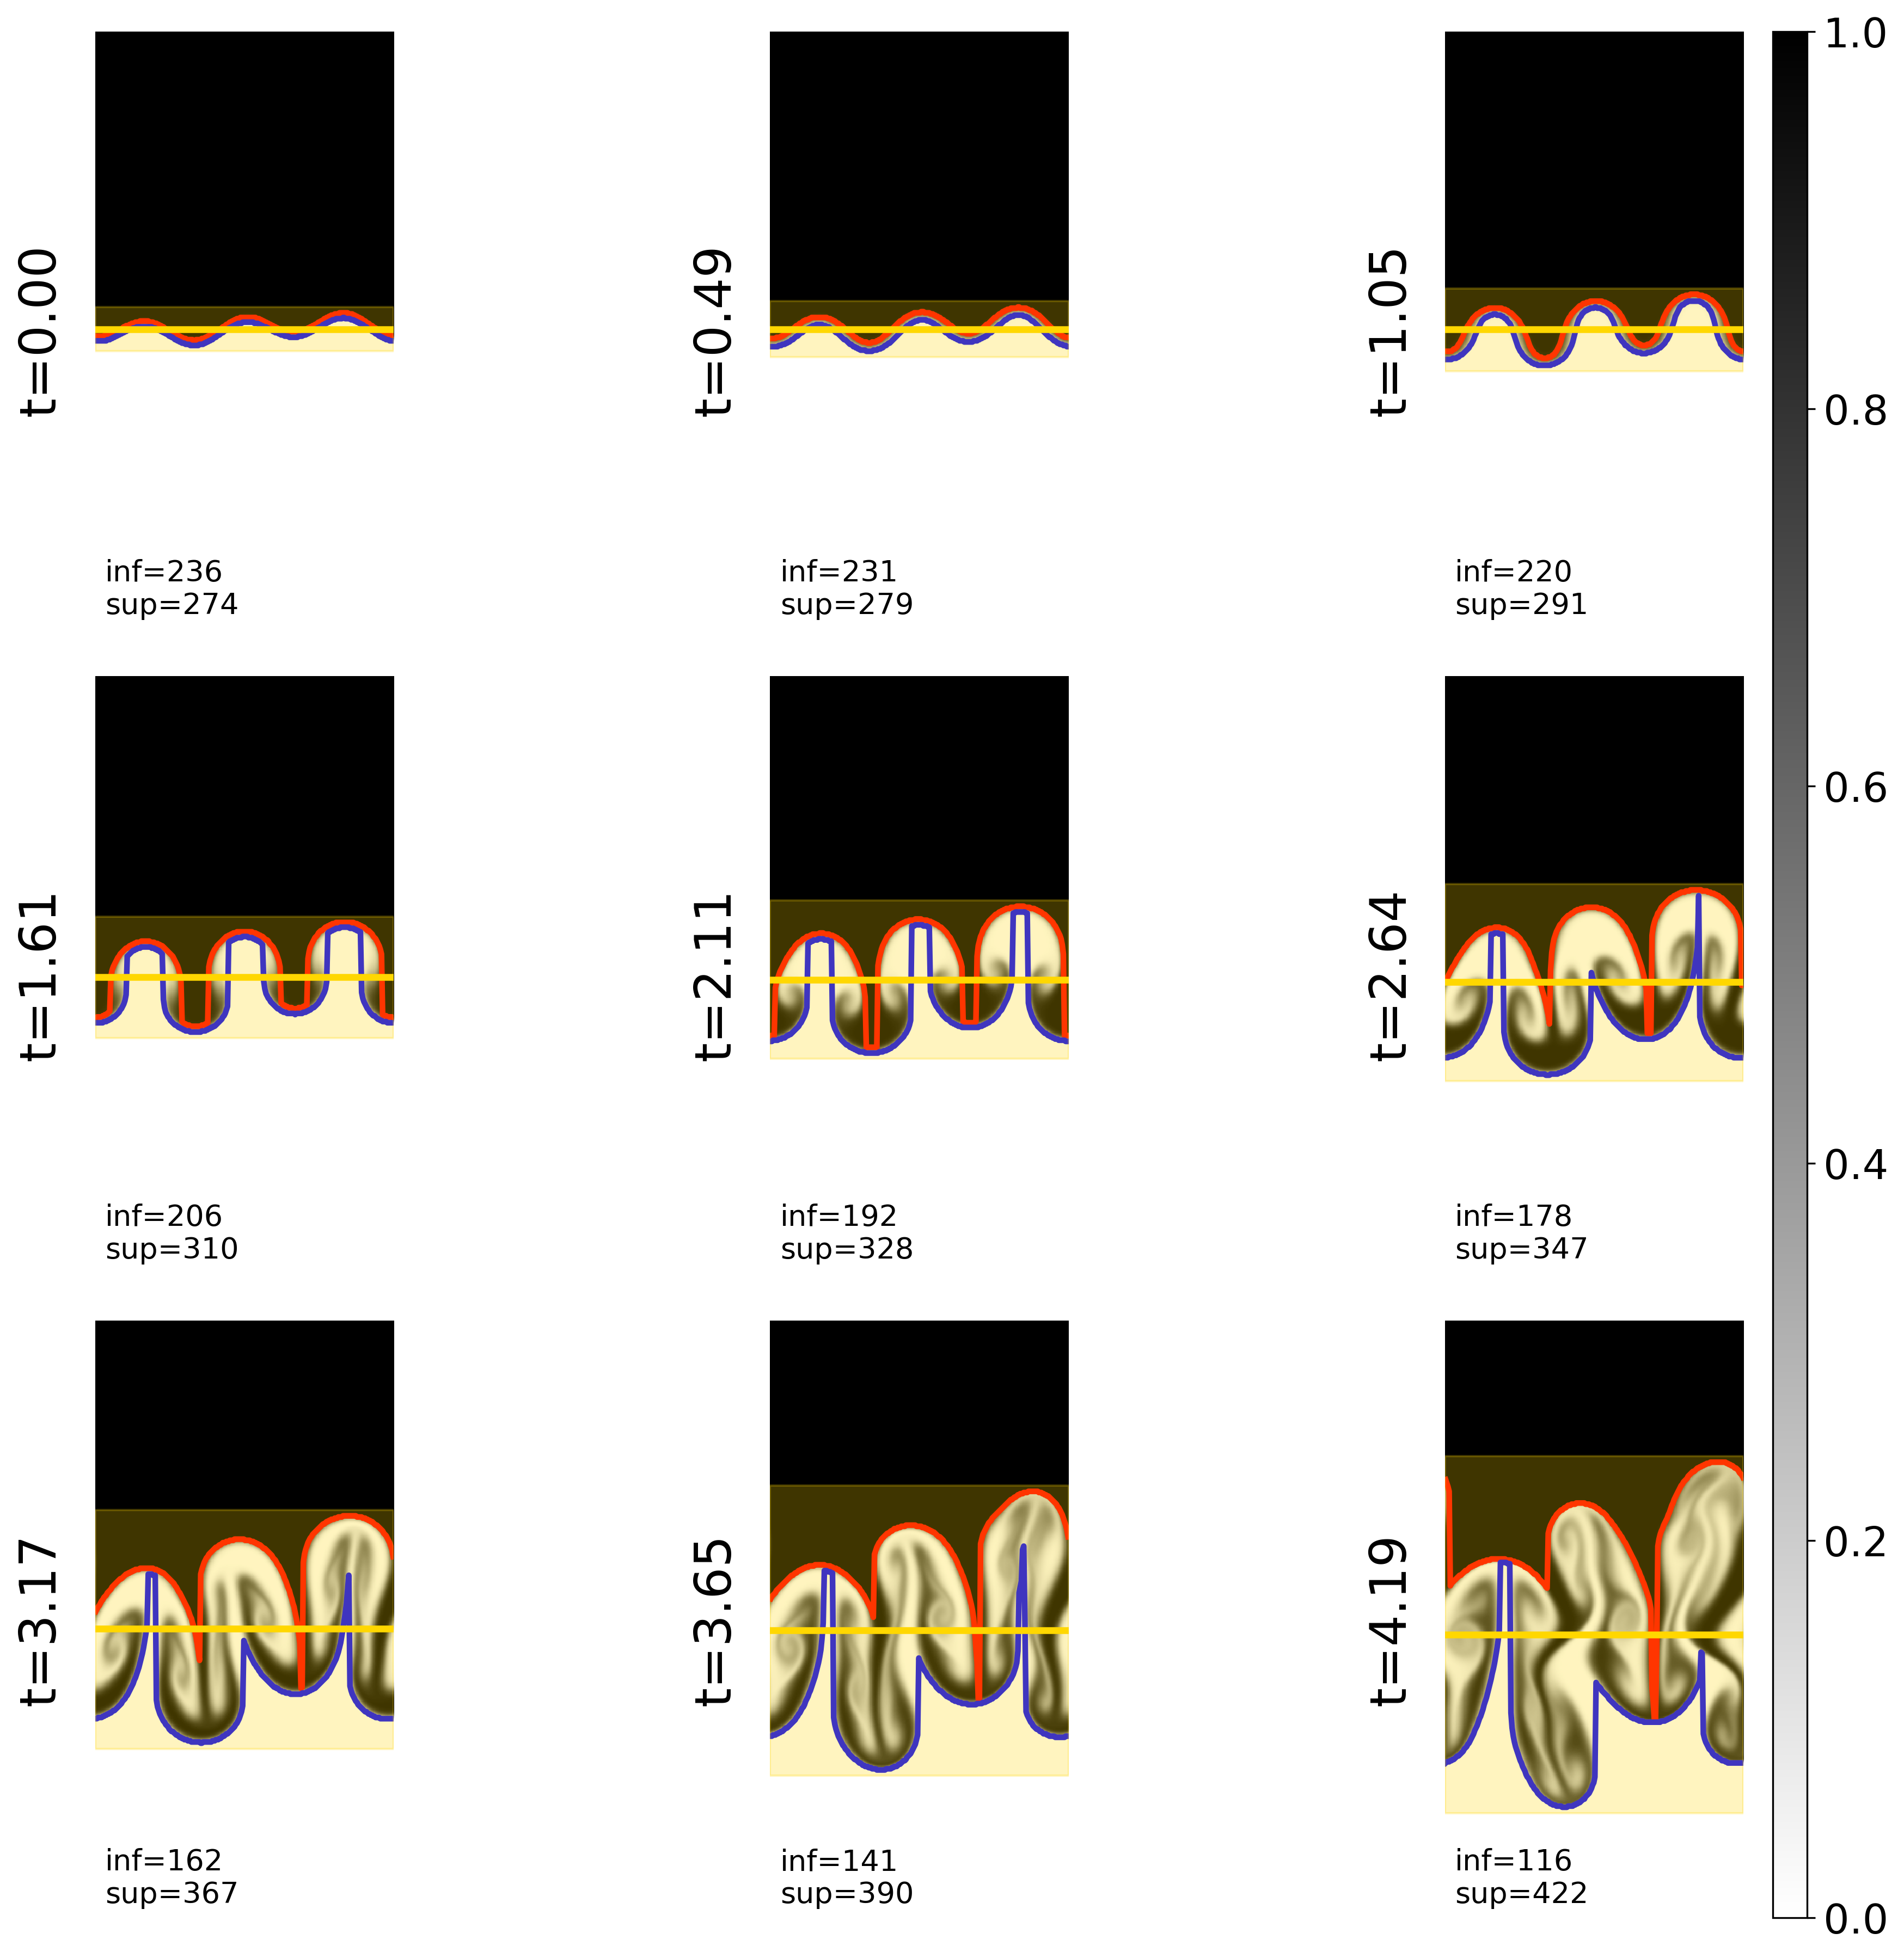
\includegraphics[width=0.65\textwidth]{figures/ch3/zone_melange.png}
\caption{Selection of the cropped field of view so that the whole mixing region remains inside the observation window.}
\label{fig:zone_melange}
\end{figure}

\subsection{Physically consistent data augmentation}

Because the data originate from numerical simulations, admissible
augmentations are constrained by the symmetries of the governing equations.
The pseudo-spectral solver uses periodic boundary conditions in the horizontal
direction, so cyclic horizontal translations preserve the physical content of
the samples. Horizontal reflection is also admissible because it corresponds to
the symmetry $x\rightarrow -x$.

The same is not true in the vertical direction. Vertical shifts modify the
position of the mixing layer relative to gravity, and vertical reflections
exchange light and heavy fluids while reversing the physical orientation of the
problem. Arbitrary rotations are excluded for the same reason. The
augmentation strategy is therefore deliberately restricted to horizontal
periodic shifts and horizontal flips.

\begin{figure}[H]
    \centering
    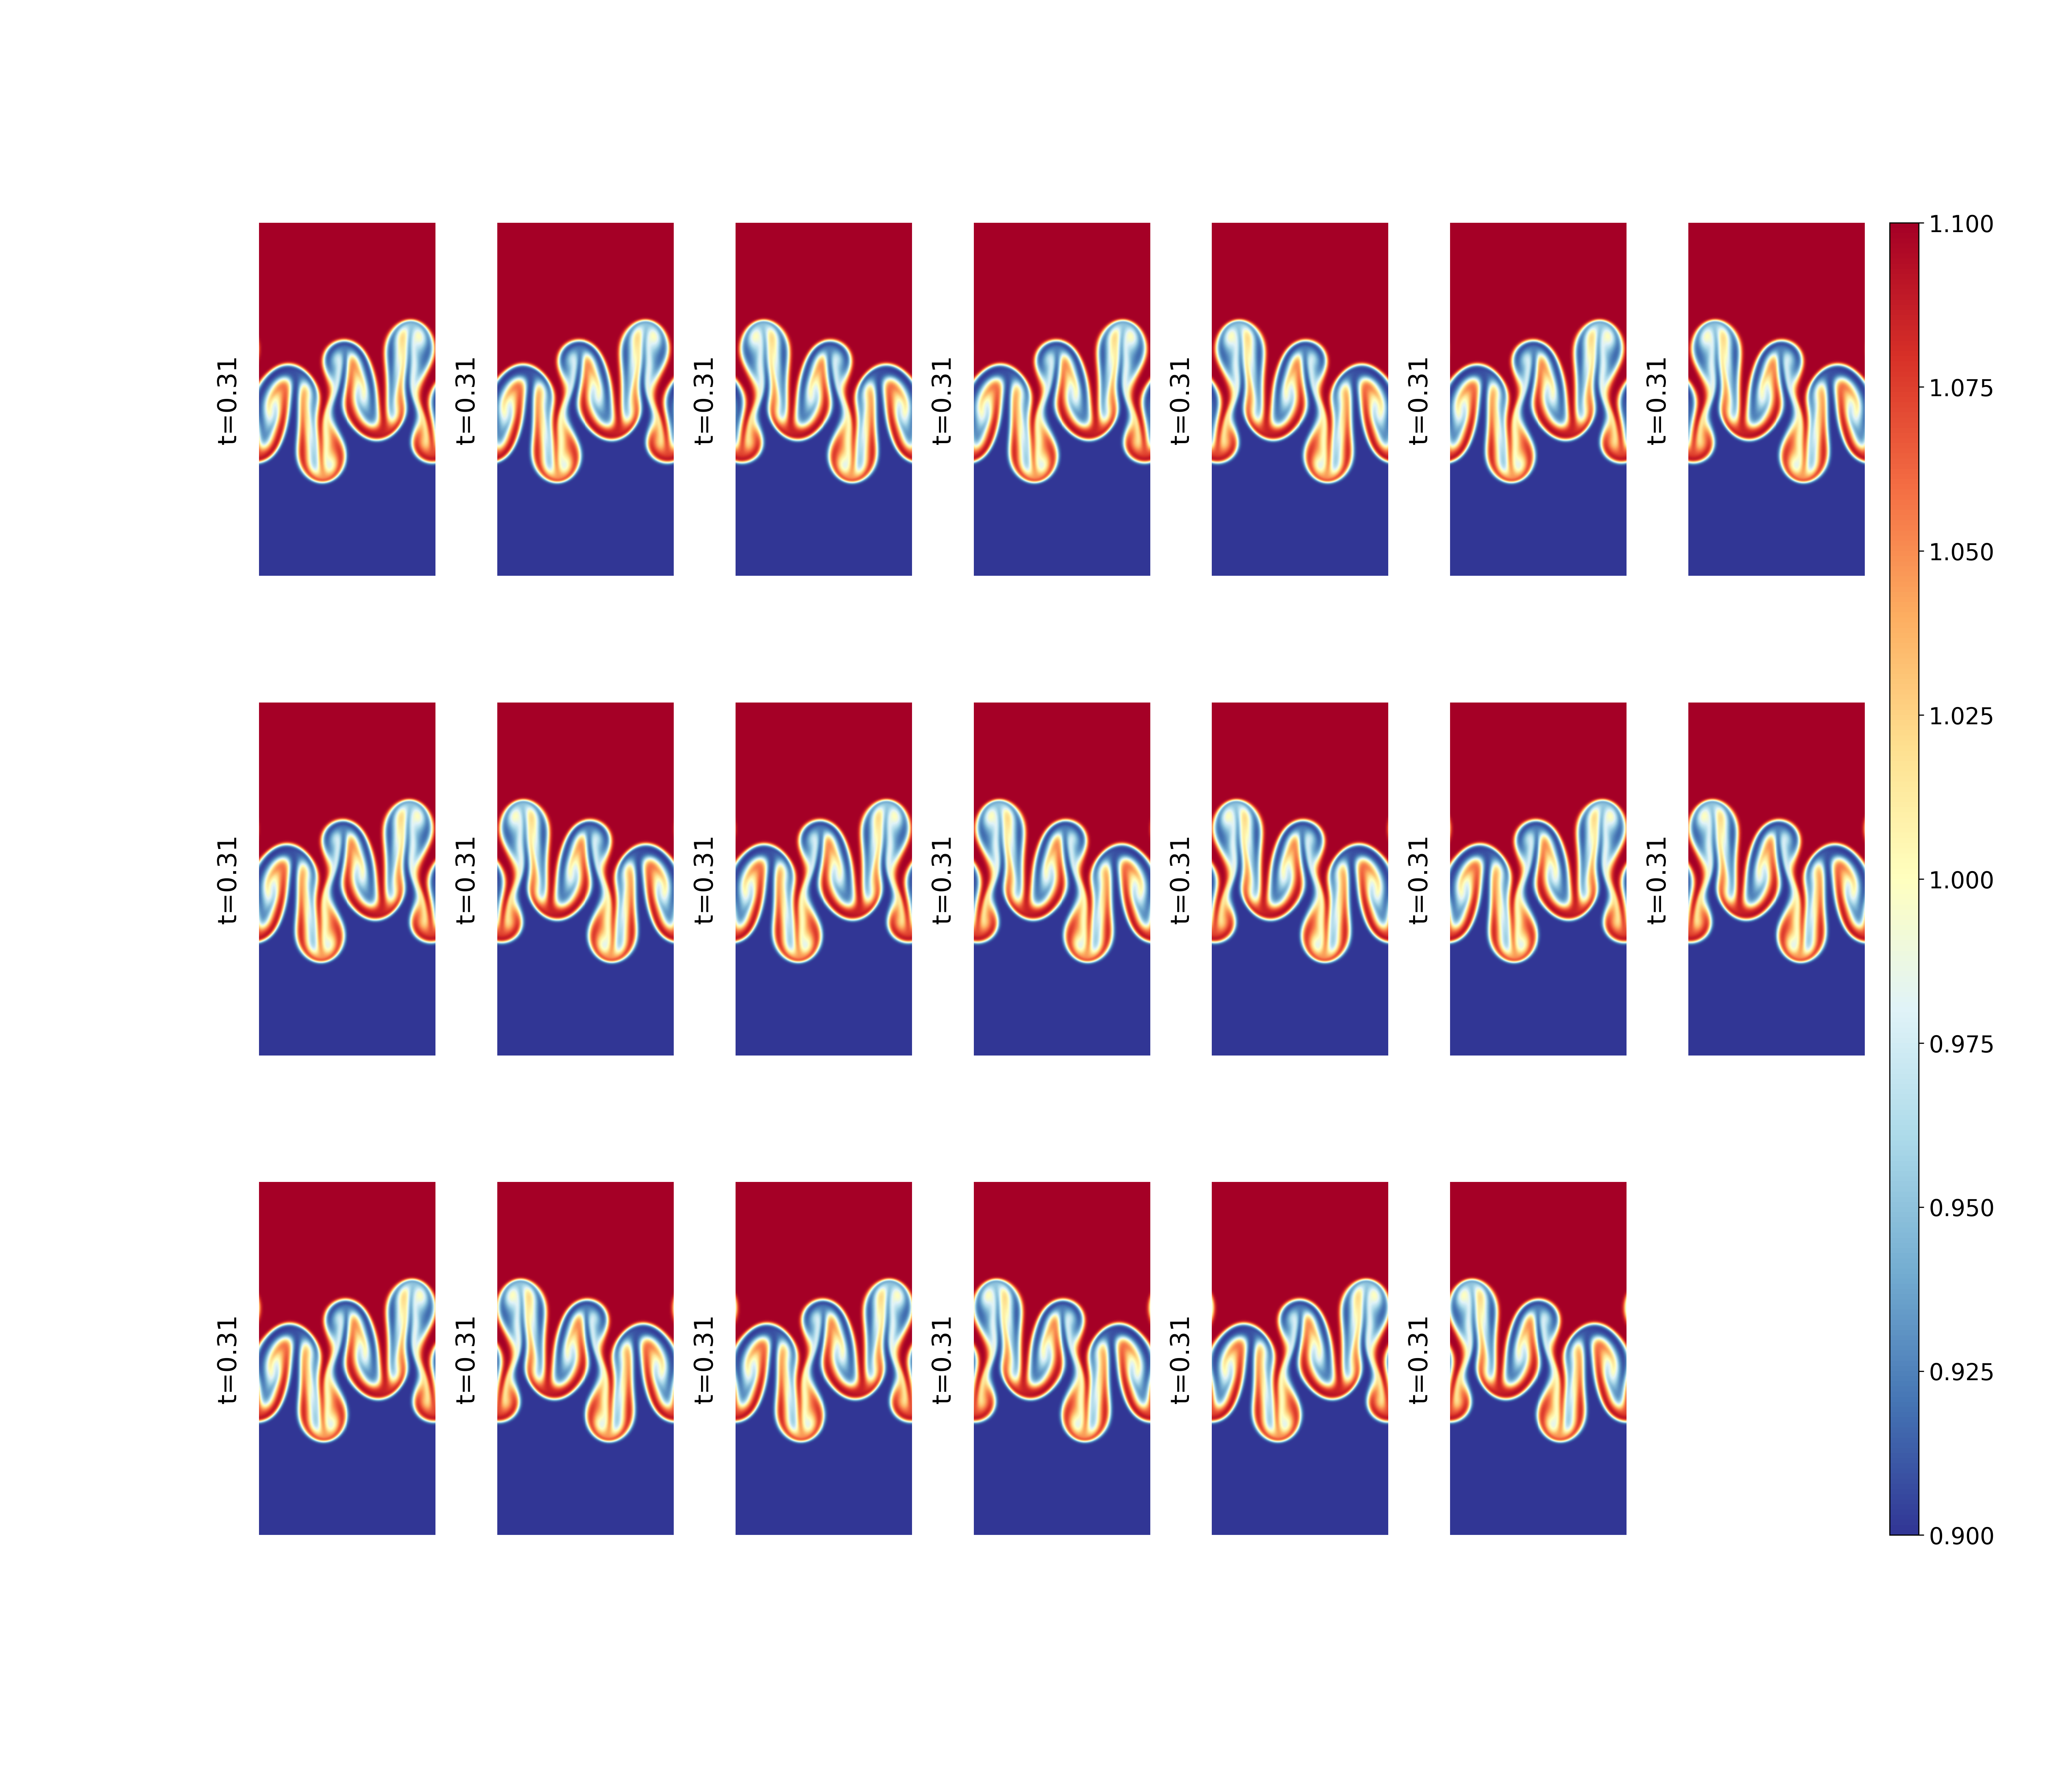
\includegraphics[width=0.95\textwidth]{figures/ch3/augmentation.png}
    \caption{Physically admissible augmentations for the RTI dataset: horizontal cyclic shifts and horizontal reflection only.}
    \label{fig:augmentation}
\end{figure}

\section{Overall Pipeline}

The complete workflow starts from Direct Numerical Simulation density fields,
applies preprocessing and physically motivated data augmentation, trains a
generative diffusion model, and evaluates generated samples against validation
data. Figure~\ref{fig:diffusion_pipeline} gives the general principle of this
surrogate modeling approach.

\begin{figure}[H]
\centering
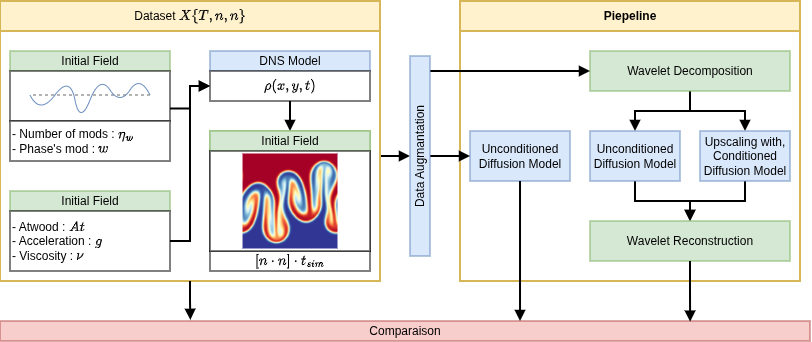
\includegraphics[width=0.95\textwidth]{figures/intro/pipeline.png}
\caption{General principle of the diffusion-based surrogate modeling approach used in this work.}
\label{fig:diffusion_pipeline}
\end{figure}

\section{Baseline Image-space Diffusion Pipeline}

The baseline model is trained directly on preprocessed two-dimensional RTI density fields. This pipeline is used as the reference against which the wavelet-based approach is compared.

The baseline implementation is organized around the script
\texttt{\_to\_move\_2D/diffusion.py} and the reusable library
\texttt{lib/diffusion\_lib}. The script plays the role of an experiment driver:
it defines the configuration, selects the computing device, loads the processed
RTI tensors, checks that the dataset shape is consistent with the model
configuration, initializes the DDPM and U-Net, launches the training loop when
required, and finally reloads the best checkpoint for visualization and
sampling.

The library separates the main components of the diffusion pipeline. The
\texttt{data\_loader} module loads the already preprocessed training,
validation, and test tensors, converts them to floating-point images, and
normalizes them in the interval $[-1,1]$. The \texttt{DDPM} module implements
the forward noising process
$x_t=\sqrt{\bar{\alpha}_t}x_0+\sqrt{1-\bar{\alpha}_t}\epsilon$, the learned
reverse denoising step, and the sampling procedure that starts from Gaussian
noise. The \texttt{UNet} module provides the time-conditioned convolutional
network used to predict the injected noise. The \texttt{training\_loop} module
contains the training logic: for each batch, a random diffusion time is sampled,
Gaussian noise is added to the clean image, the U-Net predicts this noise, and
the parameters are updated by minimizing the mean squared error between true
and predicted noise. Validation loss is used to select and save the best model
checkpoint.

The denoising network is a two-dimensional U-Net that receives a noisy density
field $\mathbf{x}_t$ together with the corresponding diffusion timestep $t$ and
predicts the injected Gaussian perturbation
$\boldsymbol{\epsilon}_{\theta}(\mathbf{x}_t,t)$. This architecture is adapted
to RTI fields because the encoder captures large-scale organization whereas the
decoder and skip connections preserve localized structures near the mixing
layer. In the implementation used here, the input has shape $(1,64,64)$, the
network contains three resolution levels, and the timestep is encoded through
a sinusoidal embedding injected at each scale.

\begin{figure}[H]
    \centering
    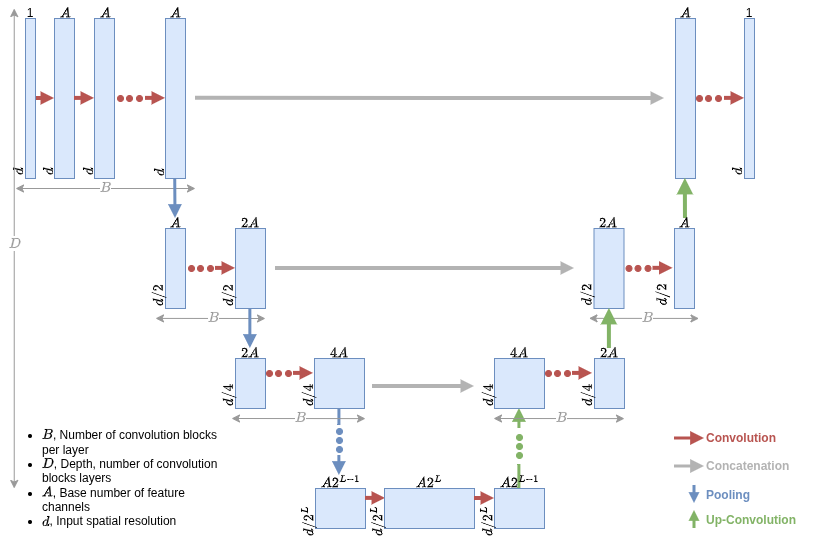
\includegraphics[width=0.82\textwidth]{figures/ch4/Unet2.drawio.png}
    \caption{Baseline U-Net denoising architecture used for image-space diffusion. The noisy field is processed jointly with a time embedding in order to predict the noise added by the forward process.}
    \label{fig:baseline_unet}
\end{figure}

At a high level, the baseline procedure can be summarized as follows:
\begin{algorithm}[H]
\caption{Baseline DDPM training and sampling procedure}
\begin{algorithmic}
\STATE Load processed RTI density fields and build training and validation loaders.
\STATE Normalize each image to the interval $[-1,1]$.
\STATE Initialize a DDPM with a time-conditioned U-Net and a linear noise schedule.
\FOR{each training epoch}
    \FOR{each batch $x_0$}
        \STATE Sample a random time step $t$ and Gaussian noise $\epsilon$.
        \STATE Build the noisy field $x_t$ using the forward diffusion equation.
        \STATE Predict $\epsilon_\theta(x_t,t)$ with the U-Net.
        \STATE Minimize $\|\epsilon-\epsilon_\theta(x_t,t)\|_2^2$.
    \ENDFOR
    \STATE Compute validation loss and save the checkpoint if it improves.
\ENDFOR
\STATE Reload the best checkpoint and generate samples by iterative reverse diffusion.
\end{algorithmic}
\end{algorithm}

\begin{figure}[H]
    \centering
    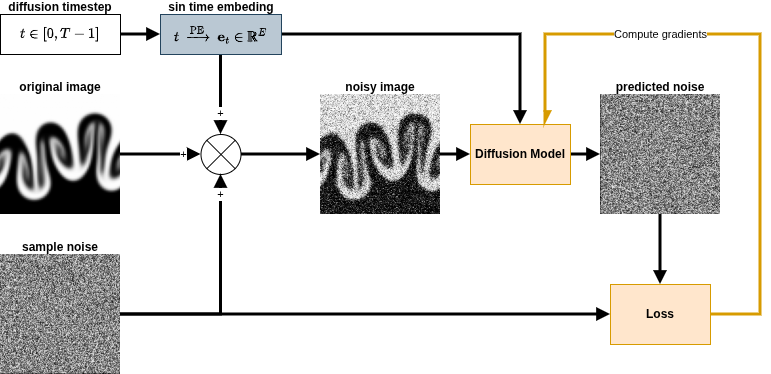
\includegraphics[width=0.82\textwidth]{figures/ch4/training_loop2.drawio.png}
    \caption{Baseline DDPM training loop. A random timestep and Gaussian perturbation are sampled for each batch, and the U-Net is trained to predict the injected noise.}
    \label{fig:baseline_training_loop}
\end{figure}

\section{Wavelet-based Diffusion Pipeline}

\section{Motivation}

The diffusion model presented in Chapter~3 operates directly on the density
fields in physical space. While this setting already provides a meaningful
baseline, it does not explicitly exploit the multi-scale structure discussed in
Chapter~2. Rayleigh--Taylor instability fields contain both large coherent
structures and fine localized fluctuations, and these components are not
equally easy to learn in pixel space. In particular, the small-scale features
associated with interface corrugations, local mixing events, and turbulent
details can be difficult to preserve when the model must simultaneously learn
the global morphology of the flow.

This observation motivates a second generative pipeline based on wavelet
coefficients. The main idea is to decompose each density field into an
approximation component, which captures the large-scale structure, and detail
components, which encode the local variations at a given resolution level. A
diffusion model is then trained not on the raw image itself, but on this
multi-resolution representation. The resulting surrogate is expected to better
capture the hierarchical organization of RTI fields and to produce samples that
preserve the dominant scales of the flow while remaining flexible enough to
reconstruct realistic fine-scale structures.

Compared with the baseline diffusion model, this approach introduces an
additional inductive bias: instead of learning the full spatial field at once,
the network learns to generate the wavelet detail coefficients conditioned on
the coarse approximation. 

An important difference also appears at the level of the prior. In the direct
diffusion model, generation starts from pure Gaussian noise having the same
spatial size as the target image. In the wavelet setting, the initial noise is
defined in coefficient space and is therefore smaller by a factor related to
the decomposition level $j$. In practice, a wavelet decomposition reduces the
resolution of the latent variable by approximately $2^j$ in each spatial
direction, so the generative model begins from a more compact prior while
still preserving the hierarchical structure needed to reconstruct the full
field.

\begin{figure}[H]
    \centering
    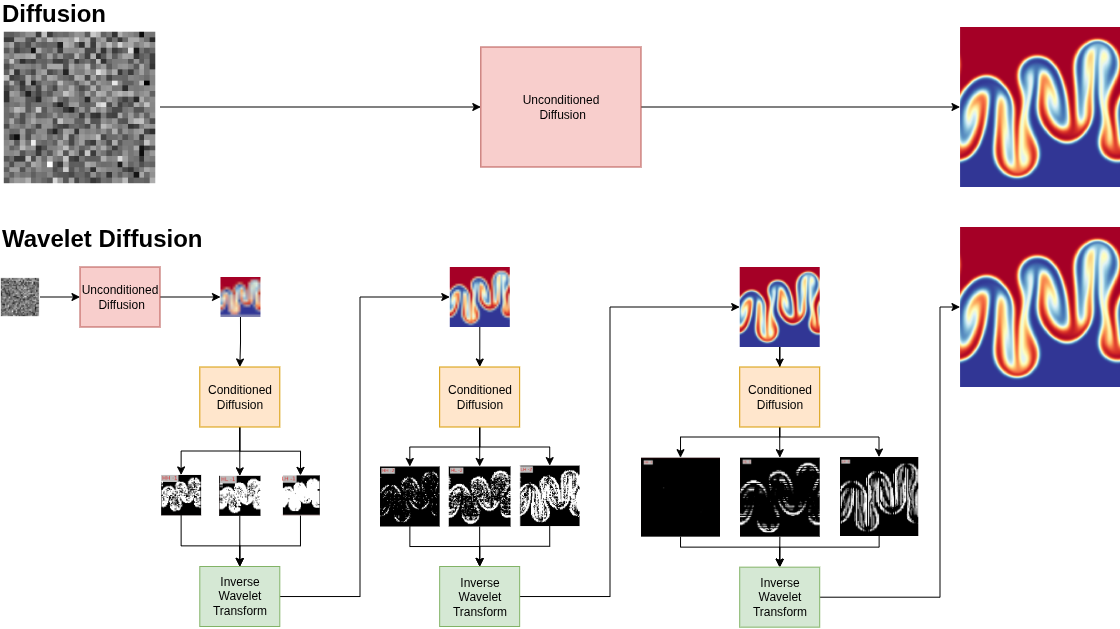
\includegraphics[width=0.95\textwidth]{figures/ch5/WaveletDiffusion.png}
    \caption{Comparison between direct diffusion and wavelet-based diffusion. In the wavelet case, the prior is defined on a lower-resolution latent representation before the inverse wavelet transform reconstructs the full field.}
    \label{fig:ch5_wavelet_diffusion_scheme}
\end{figure}





\section{Wavelet-based generative framework}

\subsection{Wavelet representation of RTI fields}

The wavelet pipeline begins with the preprocessing of the RTI dataset. The raw
density fields are first loaded from the simulation files and preprocessed
using the existing data augmentation routines. A two-dimensional discrete
wavelet transform is then applied to each image using a Daubechies-1 basis.

For a decomposition level $j$, each field is mapped to four coefficient maps:
the approximation coefficients $c_A$ and the horizontal, vertical, and
diagonal detail coefficients $c_H$, $c_V$, and $c_D$. In the implementation,
these four arrays are stacked into a tensor of shape $(N,4,H',W')$, where $N$
is the number of samples and $(H',W')$ is the spatial size of the wavelet
coefficients at the chosen level. The dataset is then split into training,
validation, and test subsets, and each split is saved independently as a PyTorch
tensor.

This representation preserves the most relevant multi-scale information while
reducing the learning problem to a structured tensor prediction task. In
practice, the decomposition also makes the notion of coarse-to-fine generation
explicit: the approximation channel plays the role of a low-frequency prior,
while the three detail channels contain the higher-frequency content that must
be synthesized.

\subsection{Conditional diffusion on wavelet coefficients}

The training data are loaded from the precomputed tensors and normalized
channel by channel using the statistics of the training split. This
normalization is important because the four wavelet channels do not share the
same numerical scale and would otherwise contribute unevenly to the
optimization process.

The model uses a conditional DDPM structure. The input to the U-Net is composed
of the approximation channel concatenated with the noisy detail channels. The
network predicts the noise applied to the detail coefficients, which means that
generation is guided by the coarse-scale information rather than being
unconditional. In other words, the model learns how to reconstruct the missing
fine-scale structure given the large-scale wavelet content.

The corresponding architecture is deliberately compact. The U-Net receives
four input channels in total, with one channel reserved for the prior
information and three channels corresponding to the target detail maps. The
network depth and the number of blocks per level remain modest so that training
is compatible with the size of the available RTI dataset. The diffusion
schedule itself follows the same principle as the baseline model, with a
discretized Markov process controlled by a linear noise schedule between
\texttt{min\_beta} and \texttt{max\_beta}.

During training, the loss is again the standard mean squared error between the
true noise and the noise predicted by the network. The model therefore learns a
denoising function conditioned on the coarse wavelet coefficients. Once
training is complete, the checkpoint and the preprocessing statistics are
stored in a configuration file so that sampling can be reproduced later without
ambiguity.

\begin{figure}[H]
    \centering
    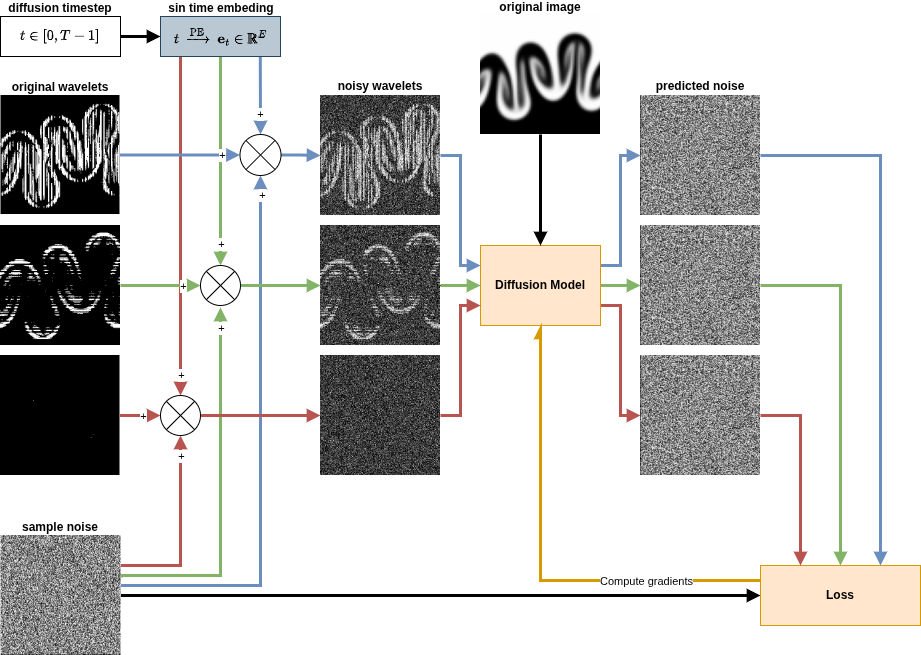
\includegraphics[width=0.88\textwidth]{figures/ch4/training_loop_conditioned.drawio.png}
    \caption{Training loop for the conditional wavelet DDPM. The approximation coefficients are kept as conditioning information, while noise is added only to the detail channels that the network must denoise.}
    \label{fig:conditioned_training_loop}
\end{figure}

% \subsection{Generation procedure}

% The generation stage loads the trained checkpoint and the associated
% normalization parameters. A batch of wavelet coefficients is sampled from the
% validation set and the approximation channel is extracted as a condition.
% Starting from the conditional prior, the DDPM iteratively denoises the target
% detail channels and produces a synthetic coefficient tensor.

% The generated coefficients are then denormalized and saved to disk. This file
% can subsequently be converted back to image space by inverting the wavelet
% transform, which makes it possible to compare the generated fields with the
% reference RTI simulations both visually and quantitatively.

% Because the generation is conditioned on the low-frequency part of an existing
% sample, the model is not asked to invent the global structure from scratch. It
% instead focuses on reconstructing plausible local details compatible with the
% coarse-scale organization of the flow. This is a natural strategy for RTI
% fields, where the large-scale morphology strongly constrains the admissible
% small-scale fluctuations.

\section{Implementation Contributions}

The implementation work conducted during the internship produced several
experimental building blocks: a configurable DDPM training script, a reusable
diffusion library, data loaders for preprocessed tensors, logging utilities,
visualization routines, checkpoint saving, and the first version of a
wavelet-conditioned diffusion pipeline. These elements made it possible to
test the direct image-space baseline and to explore the wavelet formulation.

However, the current software state is still exploratory. In particular, the
wavelet-based pipeline does not yet provide sufficiently robust or competitive
results, and some parts of the repository remain closer to research prototypes
than to a reusable package. For this reason, this work should not yet be
presented as a finalized software contribution. At this stage, the main
contribution is methodological and experimental: identifying what works for the
baseline, where the wavelet approach fails, and which parts of the pipeline
need to be stabilized before a clean external release would be meaningful.

\section{Reproducibility}

Because this internship was carried out in the CEA context, the code and data
cannot be publicly distributed in their current form. The experiments therefore
cannot be reproduced directly from a public repository. Reproducing the work
would require reimplementing the pipeline from the methodological description:
preparing equivalent RTI density fields, applying the same preprocessing and
augmentation strategy, training a DDPM baseline with the described noise
prediction objective, and then implementing the wavelet-conditioned variant.

This limitation should be kept in mind when interpreting the results. The
report provides the scientific and algorithmic details needed to understand and
reconstruct the approach, but it does not provide a complete executable
reproducibility package because of the confidentiality constraints associated
with the internship environment.

This methodology chapter detailed how the baseline and wavelet-based models are constructed. The next chapter evaluates these choices experimentally using visual, statistical, and physically motivated indicators.
